\documentclass[10pt,a4paper]{article}

% ---------------------------------------------------------------------------
% Chronicle -- the short version (VFM / new architecture, surface level)
% Compile: pdflatex CHRONICLE_SHORT.tex (twice)
% ---------------------------------------------------------------------------

\usepackage[T1]{fontenc}
\usepackage[utf8]{inputenc}
\usepackage{lmodern}
\usepackage[margin=1.9cm,top=1.7cm,bottom=1.7cm]{geometry}
\usepackage{microtype}
\usepackage{xcolor}
\usepackage{booktabs}
\usepackage{tabularx}
\usepackage{array}
\usepackage{enumitem}
\usepackage{titlesec}
\usepackage{fancyhdr}
\usepackage{amsmath,amssymb}
\usepackage{tikz}
\usetikzlibrary{arrows.meta,positioning}
\usepackage[hidelinks]{hyperref}

\definecolor{ink}{HTML}{0F172A}
\definecolor{accent}{HTML}{0F766E}
\definecolor{accent2}{HTML}{1D4ED8}
\definecolor{muted}{HTML}{64748B}
\definecolor{panel}{HTML}{F1F5F9}
\definecolor{vlm}{HTML}{7C3AED}
\definecolor{warn}{HTML}{B45309}

\color{ink}
\setlength{\headheight}{19pt}
\setlength{\parindent}{0pt}
\setlength{\parskip}{4pt}
\setlength{\emergencystretch}{2.5em}
\renewcommand{\arraystretch}{1.16}

\titleformat{\section}{\large\bfseries\color{accent}}{\thesection}{0.6em}{}
\titleformat{\subsection}{\normalsize\bfseries\color{accent2}}{\thesubsection}{0.5em}{}
\titlespacing*{\section}{0pt}{10pt}{4pt}
\titlespacing*{\subsection}{0pt}{7pt}{2pt}

\pagestyle{fancy}
\fancyhf{}
\fancyhead[L]{\footnotesize\color{muted}Chronicle --- the short version}
\fancyhead[R]{\footnotesize\color{muted}October 2026}
\fancyfoot[C]{\footnotesize\color{muted}\thepage}
\renewcommand{\headrulewidth}{0.2pt}
\renewcommand{\headrule}{\hbox to\headwidth{\color{panel}\leaders\hrule height \headrulewidth\hfill}}

\newcommand{\code}[1]{\texttt{\small #1}}
\newcommand{\kw}[1]{\textcolor{accent2}{\textbf{#1}}}
\newcommand{\vlm}[1]{\textcolor{vlm}{\textbf{#1}}}
\newcolumntype{L}{>{\raggedright\arraybackslash}X}
\newcolumntype{C}{>{\centering\arraybackslash}X}

% Minimal needspace: break the page if less than #1 remains.
\makeatletter
\newcommand{\needspace}[1]{%
  \par\penalty-100
  \begingroup
  \dimen@=#1\relax
  \ifdim\pagegoal<\maxdimen
    \advance\dimen@\pagetotal
    \ifdim\dimen@>\pagegoal
      \vfil\break
    \fi
  \fi
  \endgroup}
\makeatother

\newcommand{\panel}[1]{%
  \noindent\colorbox{panel}{%
    \begin{minipage}{\dimexpr\linewidth-2\fboxsep\relax}
    \vspace{2pt}#1\vspace{2pt}
    \end{minipage}}%
}

\newcommand{\keyidea}[1]{%
  \par\medskip\noindent\colorbox{panel}{%
    \begin{minipage}{\dimexpr\linewidth-2\fboxsep\relax}
    \vspace{2pt}\textbf{\textcolor{accent}{Key idea.}}\ #1\vspace{2pt}
    \end{minipage}}\par\medskip
}

\begin{document}

% ===========================================================================
% PAGE 1 -- THE IDEA
% ===========================================================================
\begin{center}
{\LARGE\bfseries Chronicle}\\[2pt]
{\Large\color{accent}\bfseries The short version: video-free memory}\\[4pt]
{\color{muted}\small What the new architecture does, in five minutes --- October 2026}
\end{center}

\vspace{1pt}

\panel{
\textbf{One sentence.} Chronicle compiles a video episode \emph{once} into a compact timestamped
memory --- VLM captions, a salience event ledger, a few evidence stills and an LLM-ready pack ---
then answers questions from that memory in microseconds, with \textbf{no video and no video model in
the query path}.
}

\vspace{2pt}

\begin{center}
\begin{tabularx}{\linewidth}{@{}C C C C@{}}
\toprule
{\Large\bfseries\color{accent}249\,MB} & {\Large\bfseries\color{accent}95\,KB} &
{\Large\bfseries\color{accent}0.05--0.06\,ms} & {\Large\bfseries\color{accent}0} \\
{\scriptsize source video} & {\scriptsize compiled memory} & {\scriptsize vault query, p50} &
{\scriptsize video at answer time} \\
\bottomrule
\end{tabularx}
\end{center}

\noindent
\textbf{The problem.} Every question about video normally means decoding, sampling frames and calling
a vision model again. That is slow, expensive, and coverage depends on which frames you happened to
sample. Long episodes make it worse: the video is huge, but the part you need is tiny.

\vspace{2pt}

\begin{center}
\begin{tikzpicture}[
  font=\scriptsize,
  box/.style={draw=ink!45, rounded corners=3pt, fill=white, align=center,
              inner sep=4pt, minimum height=10mm, text width=2.52cm},
  vbox/.style={box, draw=vlm!60, fill=vlm!6},
  sbox/.style={box, draw=accent!60, fill=accent!7},
  gbox/.style={box, draw=accent2!55, fill=accent2!6},
  arr/.style={-{Latex[length=2mm]}, draw=ink!60, thick}
]
\node[vbox] (video) {video episode\\249\,MB};
\node[gbox, right=6mm of video] (compile) {compile once\\seconds to minutes};
\node[sbox, right=6mm of compile] (memory) {memory at rest\\graph + vault + stills};
\node[vbox, right=6mm of memory] (question) {question\\natural language};
\node[sbox, right=6mm of question] (answer) {answer\\claim + citation + frame};
\draw[arr] (video) -- (compile);
\draw[arr] (compile) -- (memory);
\draw[arr] (memory) -- (question);
\draw[arr] (question) -- (answer);
\end{tikzpicture}
\end{center}

\noindent
\textbf{Three layers, three jobs.}

\begin{center}
\small
\begin{tabularx}{\linewidth}{@{}l L L@{}}
\toprule
\textbf{Layer} & \textbf{What it is} & \textbf{What it answers} \\
\midrule
\kw{Graph} & The index: entities, states, edges, zones, counts & where / state / who / how many \\
\vlm{Vault} & The memory: captions, coalesced events, metadata, cache & what happened / around when / describe \\
\kw{Evidence} & 480\,px WebP stills + citations & show me / prove it \\
\bottomrule
\end{tabularx}
\end{center}

\keyidea{The graph is the index; the captions and events are the recallable memory; the vault is the
fast answer engine; evidence makes it auditable. Compile once, query many times.}

% ===========================================================================
% PAGE 2 -- WHAT HAPPENS (COMPILE)
% ===========================================================================
\section{What happens: compile once}

This is the only expensive step. It runs once per clip, in the background, on first view. After it
finishes, the source video is only needed for playback and screenshots.

\begin{enumerate}[leftmargin=1.3em,itemsep=2pt]
  \item \textbf{Snapshot the source DB.} Make a consistent copy of the graph while ingest may still
        be writing.
  \item \textbf{Caption the video.} Cut it into 30\,s windows (20\,s for short clips); sample three
        frames per window; caption each frame with a VLM and synthesise a window caption. Store
        objects, actions, zone and tags.
  \item \textbf{Build the event ledger.} Read state transitions, anchors and edges; remove
        visibility noise (pan, occlusion, reacquisition) and merge repeated touches/placements into
        memory-worthy events. Pack at about 17 bytes per event.
  \item \textbf{Build the vault.} Write the packed events, string dictionary, captions, per-label
        count summaries, metadata and an answer cache into a small SQLite file.
  \item \textbf{Extract evidence.} Save a bounded set of 480\,px WebP stills: interaction strips,
        object crops and zone keyframes. No full-resolution frames are kept.
  \item \textbf{Write the pack and report.} Produce an LLM-ready pack (2k/4k/8k token budgets) and a
        single-file HTML report with a timeline and query box.
\end{enumerate}

\needspace{10\baselineskip}

\noindent
\textbf{What gets stored, and why it is small.}

\begin{center}
\small
\begin{tabularx}{\linewidth}{@{}l L r@{}}
\toprule
\textbf{Artefact} & \textbf{What it contains} & \textbf{Typical} \\
\midrule
Graph DB & entities, states, edges, zones, observations (source of truth) & 168--254\,KB \\
Vault & packed events, captions, strings, count summaries, answer cache & 28--32\,KB \\
Caption ledger & 30\,s windows: caption, objects, actions, tags, 3 frame captions & 1--2 windows \\
Event ledger & salience-coalesced state / edge / interaction events & 8--11 events \\
Evidence & 480\,px WebP stills, ranked by interaction / crop / zone keyframe & 8 frames \\
Memory pack & verified answer + ranked captions/events + evidence refs + rules & 2.4--3.0\,KB \\
Whole job dir & vault + ledger + evidence + report + pack + zip & 0.99--1.3\,MB \\
\bottomrule
\end{tabularx}
\end{center}

\noindent
A 60-minute synthetic episode with 2{,}474 events, 184 caption windows and 40 snapshots produces a
142\,KB vault. The source video is orders of magnitude larger.

\keyidea{The memory is deliberately lossy. It does not preserve every pixel; it preserves enough
\emph{timestamped meaning} to answer repeated questions, plus a pointer back to the evidence.}

\vspace{2pt}

\panel{
\textbf{Why this is more useful than the graph alone.} The graph knows \code{person
VISIBLE\_MOVING}; the caption knows ``a person walks on a sidewalk holding a cup of coffee''. Captions
also cover segments where the tracker emitted no interaction row, and their timestamps make ``around
10\,s'' a range query rather than a similarity search over one frame.
}

% ===========================================================================
% PAGE 3 -- HOW IT IS SEARCHED
% ===========================================================================
\section{How it is searched}

Query time touches only small text structures. There is no video decoding, no frame sampling and no
vision model in the default path.

\begin{center}
\begin{tikzpicture}[
  font=\scriptsize,
  box/.style={draw=ink!45, rounded corners=2pt, fill=white, align=center,
              inner sep=3pt, minimum height=9mm, text width=2.8cm},
  sbox/.style={box, draw=accent!65, fill=accent!7},
  gbox/.style={box, draw=accent2!60, fill=accent2!6},
  vbox/.style={box, draw=vlm!60, fill=vlm!6},
  arr/.style={-{Latex[length=1.9mm]}, draw=ink!60, thick},
  dasharr/.style={-{Latex[length=1.9mm]}, draw=muted, thick, dashed}
]
\node[vbox] (q) {question};
\node[vbox, right=6mm of q] (intent) {intent router\\where / when / count / ...};
\node[vbox, right=6mm of intent] (vault) {deterministic vault\\lookup + cache};
\node[sbox, right=6mm of vault] (answer) {answer + citations\\+ evidence + frame chip};
\node[gbox, below=6mm of vault] (graph) {graph fallback\\2-hop GraphRAG};
\node[gbox, right=6mm of graph] (qwen) {optional Qwen\\phrasing over text};
\draw[arr] (q) -- (intent);
\draw[arr] (intent) -- (vault);
\draw[arr] (vault) -- node[above,font=\tiny]{hit} (answer);
\draw[arr] (vault) -- node[right,font=\tiny]{miss} (graph);
\draw[arr] (graph) -- (qwen);
\draw[dasharr] (qwen) -- (answer);
\end{tikzpicture}
\end{center}

\noindent
\textbf{What the router understands:} where / when / around / before / after / count / holding /
inventory / yes-no / keyword. It resolves the entity and time, looks up captions and events, and
returns a deterministic answer with a citation. Paraphrases hit a canonical answer cache.

\subsection*{Trace: ``What happened around 10 seconds?''}

\begin{enumerate}[leftmargin=1.35em,itemsep=1pt]
  \item Parse the intent \code{around} and the time \(t=10\)\,s.
  \item Find the caption windows and coalesced events covering that range in the vault.
  \item Rank the nearest window/events and attach citation timestamps.
  \item Compose the answer deterministically; cache the canonical form.
  \item Attach an evidence still if one is within 8\,s, and render the \code{frame @ t} chip.
  \item If the vault has no match, ask the graph (state/edges) and label the answer
        \code{graph-fallback}.
\end{enumerate}

\noindent
\textbf{Cost of each path} (30-question internal regression suite):

\begin{center}
\small
\begin{tabularx}{\linewidth}{@{}L r r r@{}}
\toprule
\textbf{Path} & \textbf{Accuracy} & \textbf{p50} & \textbf{Video at query} \\
\midrule
Deterministic vault & \textbf{30/30} & \textbf{0.05--0.06\,ms} & no \\
Qwen 7B over the memory pack & \textbf{30/30} & 1.07\,s & no \\
Original graph + Qwen 7B & 14/30 & 0.85\,s & yes \\
9-frame contact sheet + Qwen2.5-VL & 7/30 & 4.46\,s & yes (19.24\,MB) \\
\bottomrule
\end{tabularx}
\end{center}

\needspace{7\baselineskip}

\noindent
\textbf{Counts are answered honestly.} The vault reports three numbers per label: \code{tracks}
(raw ids, upper bound), \code{peak} (most same-label boxes in one frame, lower bound) and
\code{physical} (after removing cross-label duplicates and one-frame transients, an estimate). On the
cook clip, four ``bowl'' tracks resolve to \textbf{zero physical bowls} because two were plates
double-labelled and one was a one-frame detection.

\keyidea{The default answer path has no model in it. That makes it reproducible, cheap and fast on
stage; the LLM is an optional phrasing layer, and the graph is the structured fallback.}

% ===========================================================================
% PAGE 4 -- WHY IT WINS / LIMITS / PITCH CARD
% ===========================================================================
\section{Why it wins, and what to say}

\begin{center}
\small
\begin{tabularx}{\linewidth}{@{}l L@{}}
\toprule
\textbf{Claim} & \textbf{Proof} \\
\midrule
Cheap to keep & 249\,MB video \(\rightarrow\) 95\,KB memory; whole job dir still under 1.3\,MB \\
Fast to query & 0.05--0.06\,ms vault p50; 0.89\,ms cold on a 15-minute walk \\
No video at query & captions, events, counts and evidence answer the question; video is for playback only \\
Auditable & every answer carries a timestamped citation and an evidence still; frame chip seeks to it \\
Offline and robust & the deterministic path works with no LLM; the graph answers when captions miss \\
Coverage & caption windows cover the whole episode, including segments with no interaction row \\
\bottomrule
\end{tabularx}
\end{center}

\noindent
\textbf{Honest limits (say these before judges ask).} Captions are lossy; fine motion, small text,
audio and subtle social cues are lost. The VLM can hallucinate detail. Counts are estimates, not
hand-labelled ground truth. Caption-first clips without a graph have no state/edge fallback. The
30-question suite is internal, not a public benchmark. The system is strongest on ``what happened /
where / when / how many / what is X holding'', weakest on ``why / exactly how / tiny object''.

\vspace{2pt}

\section*{Judge Q\&A cheat sheet}

\begin{itemize}[leftmargin=1.2em,itemsep=2pt]
  \item \textbf{``Isn't this just captions?''} No: captions + a salience event ledger + graph counts
        + deterministic intents + evidence. Captions alone cannot answer ``when'', ``how many'' or
        ``where'' cleanly.
  \item \textbf{``Why not just use a video LLM?''} We do, at compile time. The win is query time: the
        baseline re-samples the video for every question; we compile once and answer in microseconds.
  \item \textbf{``Is 30/30 a benchmark?''} No --- it is an internal regression suite covering
        location, temporal, count, negation and paraphrase cases. External benchmarks are next.
  \item \textbf{``What is lost?''} Fine motion, audio, tiny text, some rare objects. Evidence and
        citations make errors inspectable, not invisible.
  \item \textbf{``Does it need the video?''} No. That is the whole point; the source is kept only for
        playback and screenshots.
\end{itemize}

\vspace{2pt}

\section*{The 60-second demo}

\begin{enumerate}[leftmargin=1.35em,itemsep=1pt]
  \item Show the 15-minute, 249\,MB video and the 95\,KB memory side by side.
  \item Ask ``where are my keys?''. Show the answer, timestamp and frame chip.
  \item Ask ``what happened around 10 minutes?''. Show the caption window and evidence still.
  \item Ask a count question. Show \code{tracks / peak / physical} and the dedup example.
  \item Stop the LLM and repeat a query: the deterministic answer still cites the graph.
  \item Ask something the vault misses; show the labelled \code{graph-fallback} answer.
\end{enumerate}

\vspace{3pt}

\panel{
\textbf{One line to close.} ``Every question about a long video normally means re-watching it. We
compile the video into a 95\,KB memory once, then answer in under a millisecond, with evidence ---
and the video is optional.''
}

\vspace{4pt}

\begin{center}
{\color{muted}\small Not a replacement for a video LLM --- the memory layer that makes one unnecessary
for repeated questions.}
\end{center}

\end{document}
